% CareCompanion — ICISS 2027 camera-ready, Springer LNNS (llncs.cls v2.21)
\documentclass[runningheads]{llncs}

\usepackage[T1]{fontenc}
\usepackage{graphicx}
\usepackage{booktabs}
\usepackage{color}
\usepackage{hyperref}
\renewcommand\UrlFont{\color{blue}\rmfamily}

\begin{document}

\title{CareCompanion: A Caregiver-Mediated Android\\System for Older Adults, with Fail-Honest Alerting}
\titlerunning{CareCompanion: Caregiver-Mediated Care with Fail-Honest Alerting}

\author{Devanshi Pandey \and Suyash Humne \and Deon Menezes \and\\
Sonali Wankhede \and Balwant Kumar Singh}
\authorrunning{D. Pandey et al.}

\institute{K.~J.~Somaiya School of Engineering, Somaiya Vidyavihar University,\\
Mumbai, India\\
\email{\{devanshi.pandey,suyash.humne,deon.m,sonali.w,balwantkumar\}@somaiya.edu}}

\maketitle

\begin{abstract}
Mobile applications that help older adults manage medication and summon help are
typically evaluated on the legibility of the older adult's interface. We argue that a
second property matters at least as much and is rarely examined: whether the system
tells the truth when it fails. We present CareCompanion, an implemented Android system
for caregiver-mediated elder care built on three design commitments. First, an
asymmetric dual-surface architecture places all configuration on the caregiver's device
and leaves the older adult a zero-configuration surface of seven destinations; measured
from the source, the elder surface has a median declared text size of 20\,sp against
13\,sp on the caregiver surface, and every primary control equals or exceeds 64\,dp
against a 48\,dp platform minimum. Second, out-of-band device binding resolves an
identity gap created by federated sign-in: a single-use numeric code issued to the
caregiver binds the older adult's device to a care profile, replacing phone-number
matching, which federated identity does not supply. Third, fail-honest alerting requires
the interface never to assert an outcome it has not observed; we state precisely which
event each confirmation reflects, and show that our own first implementation violated
this rule. As a single-system, single-rater case study, a structured audit of the
feature-complete system found 13 defects, of which 8 would have failed with no
user-visible signal, including two features that were written, stored, and never
delivered. We report the taxonomy, the mechanisms that address each class, and an
explicit account of what remains unevaluated: no user study has been conducted, and the
binding code is not yet rate-limited.

\keywords{Elder care \and Mobile health \and Caregiver-mediated systems \and
Accessibility \and Dependability \and Android \and Case study.}
\end{abstract}

\section{Introduction}

India is experiencing rapid population ageing, creating growing demand for accessible
and scalable elder-care support. The United Nations Population Fund projects that
India's population aged 60 and over will grow by 134\% between 2022 and 2050, and the
population aged 80 and over by 279\%~\cite{unfpa}. Digital access, however, remains
uneven across age groups: although mobile-phone use is widespread nationally, internet
use declines substantially with age~\cite{dfi}, and among older adults in rural India
--- particularly women --- shared handsets and limited digital literacy are the norm
rather than the exception~\cite{chakraborty,khare}.

Medication non-adherence is a significant concern among older adults managing chronic
conditions and polypharmacy. Randomised evidence suggests mobile reminder tools help but
do not solve the problem: a trial of a drug-management application among older adults
with polypharmacy reported improved adherence and reduced readmission~\cite{poor}, while
a systematic review of reminder technologies for home-dwelling older citizens reports
beneficial effects for some outcomes but emphasises that the overall evidence remains
heterogeneous~\cite{salmensuu}.

The usability literature is clear about what makes an interface hard for an older adult.
Small text is repeatedly the single most-cited barrier; touch targets are too small for
reduced dexterity; icons are misread; and navigation depth exceeds working
memory~\cite{awan,elguera,liu}. Design guideline syntheses converge on enlarged type,
enlarged targets, shallow navigation, and error tolerance~\cite{gomez,amouzadeh}.

What this literature largely assumes is that the older adult is the person configuring
the system. In practice, care is dyadic. Quinn et al.\ found in a dyad usability study
that most interaction occurred between caregiver and older adult rather than the older
adult alone~\cite{quinn}, and dyadic digital health modules are now designed explicitly
around shared care~\cite{benmessaoud}. If the caregiver is doing the configuring, then
the older adult's surface does not need to be a simplified version of a management
application. It can be a different application altogether.

A second assumption is more consequential and, we argue, under-examined: that when the
system reports success, it has succeeded. Emergency and reminder paths on mobile
platforms are unreliable in ways the application can observe but frequently does not
check. Android's Doze and App Standby defer alarms and network access during
idle~\cite{doze}, and original-equipment-manufacturer power management is more
aggressive still. Push delivery depends on connectivity that an older adult at home may
not have. An interface that renders a green tick on an emergency alert it never
delivered is not merely unhelpful; in the one situation the system exists for, it is
actively harmful.

\subsubsection{Contributions.} This paper makes four contributions.

\begin{itemize}
\item An \emph{asymmetric dual-surface architecture} for caregiver-mediated elder care,
in which configuration authority and interface complexity are deliberately unequal
across two clients over one care record, with the asymmetry measured from the
implementation rather than asserted (Sections~\ref{sec:asym} and~\ref{sec:conf}).

\item \emph{Out-of-band device binding}, a single-use code that binds a device to a care
profile. We show that migrating to federated identity silently breaks phone-number-based
linking, and that an out-of-band code is a simple, auditable repair. We give its threat
model explicitly, including the properties it does \emph{not} yet have
(Section~\ref{sec:binding}).

\item \emph{Fail-honest alerting}: a discipline in which the interface never asserts an
unobserved outcome. We name the exact event each confirmation reflects, and report that
our own first implementation of this very screen violated the rule
(Section~\ref{sec:honest}).

\item An \emph{empirical defect taxonomy} from a structured audit of the feature-complete
system, showing that silent failures dominate. We present this as a single-system,
single-rater case study throughout (Section~\ref{sec:defects}).
\end{itemize}

We are explicit about scope. This is a systems and design-contribution paper. We report
conformance, interaction cost, and defect data measured from the artefact. We have not
run a user study, and we make no usability, adherence, or clinical claim
(Section~\ref{sec:limits}).

\section{Related Work}

\subsection{Age-Friendly Mobile Interface Design}
Systematic reviews of mobile design for older adults consistently identify text size,
target size, icon interpretability, and navigation complexity as the dominant barriers.
Awan et al.\ applied an analytical hierarchy process to prioritise usability barriers and
ranked small font and screen size highest~\cite{awan}. Elguera Paez and Zapata Del R\'io
catalogue challenges across the literature~\cite{elguera}. Gomez-Hernandez et al.\ derive
design guidelines through thematic synthesis~\cite{gomez}, and Amouzadeh et al.\ provide
a recent consolidation of age-friendly design recommendations~\cite{amouzadeh}. Liu et
al.\ review interface and persuasive feature design in mobile health applications for
older adults~\cite{liu}. Our elder surface is an implementation of this consensus; our
contribution is not the guidelines but the demonstration that offloading configuration
to a second surface is what makes conformance affordable.

\subsection{Medication Reminder and Adherence Systems}
Poorcheraghi et al.\ report a randomised controlled trial of a mobile drug management
application among older adults with polypharmacy, finding improved adherence and reduced
hospital readmission~\cite{poor}. Salmensuu et al.\ systematically review reminder
technologies for home-dwelling older citizens~\cite{salmensuu}. Wiecek et al.\ report
real-world engagement and adherence evidence for older adults~\cite{wiecek}. These
studies evaluate outcomes; they do not generally report whether reminders were delivered
by the operating system as scheduled, which Section~\ref{sec:arming} treats as a
first-class engineering problem.

\subsection{Dyadic and Caregiver-Mediated Health Systems}
Quinn et al.\ conducted a dyad usability study of a mobile application used by older
adults together with informal caregivers, observing that interaction was predominantly
caregiver-mediated~\cite{quinn}. Benmessaoud et al.\ designed a dyadic digital health
module for chronic disease shared care~\cite{benmessaoud}. Nimmanterdwong et al.\ review
human-centred design practice in mobile health for older adults~\cite{nimman}. This work
establishes the dyad as the unit of design. We extend it architecturally: rather than one
application used by two people, we build two surfaces of deliberately unequal complexity
over one access-controlled record.

\subsection{Personal Emergency Response Systems}
Personal emergency response systems have a long history and a well-documented failure
mode: Hamill et al.\ report call-centre estimates attributing as much as 85\% of calls to
false alarms, largely accidental activations~\cite{hamill}. This motivates our cancellable
grace period. The complementary failure --- an alarm the user believes was raised but
which never reached anyone --- is less discussed in that literature, and is what
fail-honest alerting addresses.

\subsection{Gap}
Across these strands, interface legibility for the older adult and outcome efficacy are
well covered; delivery honesty and deployability under platform policy are not. Few
studies in the reviewed elder-care literature explicitly report a taxonomy of silent
implementation failures, or treat application-store permission policy as an architectural
design constraint on the emergency path.

\section{System Design}

\subsection{Asymmetric Dual-Surface Architecture}
\label{sec:asym}

The system presents two Android surfaces backed by one record. To avoid ambiguity we fix
a counting rule and use it throughout: a \emph{navigation destination} is one entry
registered in the client's navigation graph, counted from the source. By that rule the
caregiver surface has 20 destinations and the elder surface has 7, plus a one-time
binding screen reached only at set-up and not part of the running surface.

\begin{figure}[tb]
\centering
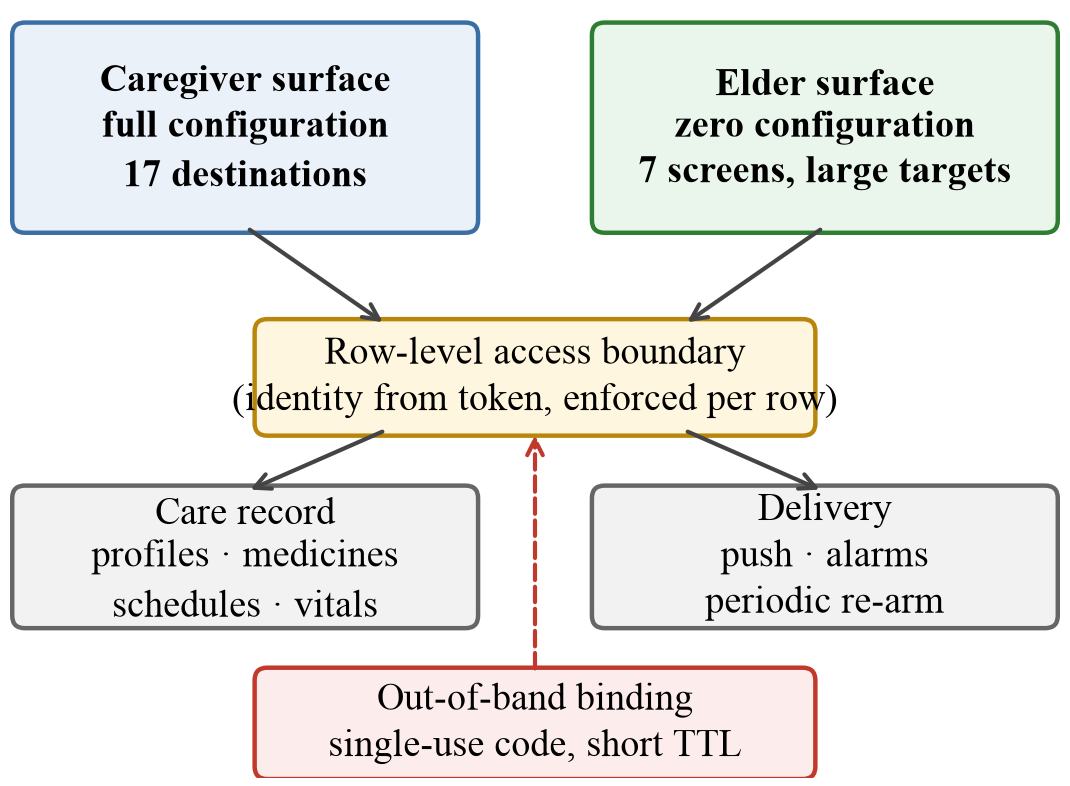
\includegraphics[width=0.62\textwidth]{fig_arch.png}
\caption{System structure. Two clients of deliberately unequal complexity share one care
record behind a per-row access boundary that derives identity from the caller's token.
The out-of-band binding step (bottom) establishes which physical device belongs to which
older adult, a link federated sign-in does not provide.}
\label{fig:arch}
\end{figure}

The caregiver surface carries the full management vocabulary: profiles, medicines,
schedules, reminders, contacts, vitals, adherence history, shortcuts, shared access, and
an emergency monitor. The elder surface carries a home screen, an alarm control, today's
medicines, contacts, vitals entry, media shortcuts, and a settings screen containing
three controls. Contacts on the elder surface are photo-first: family members are
presented as photographs rather than text labels, so recognition does not depend on
reading a name.

The asymmetry is the design. Because no configuration occurs on the elder surface, that
surface has no forms to validate, no destructive actions to guard, no navigation deeper
than two levels, and no state the older adult can corrupt. This is what makes generous
type and target sizing affordable: a screen that must accommodate a scheduling form
cannot also give every control 96\,dp of height. Section~\ref{sec:conf} quantifies the
resulting difference.

Both surfaces authenticate with a federated identity provider and address the same record
through a per-row access boundary. Thirty-three row-level policies across seventeen tables
derive the caller's identity from the verified token rather than from any client-supplied
parameter, so a modified client cannot widen its own visibility. All privileged
transitions --- creating a profile, issuing a code, redeeming one, changing another
member's access --- are server-side routines rather than client writes.

\subsection{Out-of-Band Device Binding}
\label{sec:binding}

Elder-care systems must answer a question ordinary applications do not: which physical
device belongs to the person being cared for? The caregiver creates the profile, so the
profile cannot identify its subject by who created it.

Our first implementation matched on phone number. The caregiver entered the older adult's
number; when a device signed in with that number, the two were linked. This works under
telephone-number-based authentication and fails completely under federated sign-in, which
returns an email address and a provider subject identifier and no telephone number at all.
After migrating to federated sign-in, the stored telephone number for every account was
the empty string, and the matching predicate could never be satisfied. The failure was
silent: links were recorded in a pending state, and the resolution routine compared an
empty string against a real number indefinitely. Section~\ref{sec:defects} returns to this
as an instance of a general hazard.

The repair is an out-of-band binding primitive. The caregiver requests a six-digit code
bound to the profile; the code is single-use and expires after seven days. On the older
adult's device, after federated sign-in, entering the code claims the profile for that
account. The channel by which the code travels is deliberately unspecified --- spoken
aloud in the same room, sent over any messaging application, or typed by the caregiver on
the older adult's device --- because the caregiver is present in the overwhelming majority
of set-ups~\cite{quinn}.

\subsubsection{Threat model, stated precisely.}
We state what the primitive does and does not guarantee, because an earlier draft of this
work described the code as ``short-lived'', which a seven-day lifetime does not justify.

\emph{What holds.} Redemption is an authenticated operation: the endpoint rejects any
caller without a verified federated token and a provisioned account, so an anonymous
attacker cannot reach the code-checking path at all. The code is single-use, so a shared
code cannot be replayed. A profile already bound to one account cannot be silently
rebound. Unknown and expired codes return an identical message, so those two cases cannot
be distinguished by response.

\emph{What does not hold, and is future work.} The code space is $10^6$. Over a seven-day
window, an authenticated attacker who could issue requests without restriction would face
an expected $5\times10^5$ attempts to hit a specific live code, and far fewer to hit
\emph{any} live code once many are outstanding --- a birthday-style exposure that grows
with deployment size. The system implements \emph{no attempt limit, no lockout, and no
per-account or per-address rate limiting}; we verified this by inspection of all fifteen
database migrations. Redemption is also not atomic: the routine reads the code row and
later updates it without row-level locking, so two concurrent redemptions of the same code
can both observe it as unredeemed. Finally, an already-redeemed code returns a message
distinct from the unknown-code message, which is a partial enumeration oracle, narrower
than the one the uniform expiry message closes but real.

None of these has been adversarially tested. The mitigations are standard and
inexpensive --- a counter with exponential back-off per account, \texttt{SELECT \ldots{}
FOR UPDATE} on the code row, a shorter lifetime, a larger code space, and a uniform
failure message --- and we report their absence rather than describing the primitive as
secure. The same primitive, parameterised by an access level, later replaced the equally
broken caregiver-invite path, which depended on the same telephone-number assumption.

\subsection{Fail-Honest Alerting}
\label{sec:honest}

We adopt a single rule: the interface never asserts an outcome it has not observed.
Applied to the emergency path, this produces the machine in Fig.~\ref{fig:honest}.

\begin{figure}[tb]
\centering
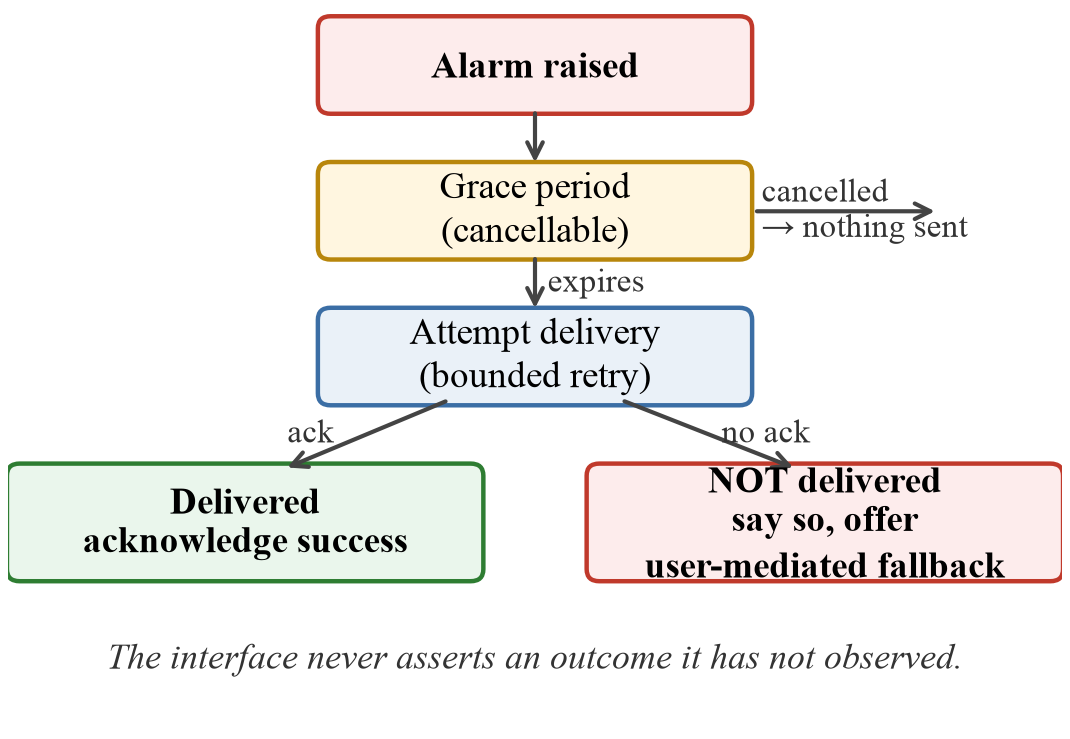
\includegraphics[width=0.62\textwidth]{fig_failhonest.png}
\caption{The emergency path. A cancellable grace period addresses accidental activation,
which dominates personal emergency response system traffic~\cite{hamill}. The terminal
states are distinguished by an observed server acknowledgement, not by having attempted
delivery.}
\label{fig:honest}
\end{figure}

Pressing the alarm control begins a five-second cancellable grace period. This is a direct
response to the dominant failure mode of personal emergency response systems --- Hamill et
al.\ report estimates of up to 85\% of call-centre traffic arising from accidental
activation~\cite{hamill} --- and it costs a genuine emergency five seconds.

\subsubsection{What each confirmation actually observes.}
A reviewer of an earlier version rightly pressed us on this, and the honest answer is
narrower than the phrase ``the alert was delivered'' suggests. The client makes up to
three attempts, with increasing delay, to write an alert row to the server; that row is
what the server's fan-out and push machinery consume. The confirmation shown to the older
adult is permitted by exactly one event: \textbf{the server acknowledged persistence of
the alert record}. It is not push acceptance by the push provider, not delivery to a
caregiver device, not display of a notification, and not acknowledgement by a human
caregiver. Correspondingly, the failure state is entered when that write was not
acknowledged after the final attempt, and it then states plainly that the alarm was not
delivered and presents two large controls: one opens the device's own messaging
application with the emergency text and a location link pre-composed, and one dials the
primary contact.

This distinction is not pedantic. The caregiver-facing acknowledgement --- a human
marking the event as seen --- exists in the data model and is visible on the caregiver's
monitor, but it is not currently propagated back to the older adult's device. Closing
that loop, so that the elder surface can distinguish ``your family's phone received this''
from ``your family has seen this'', is the single most valuable extension of the
discipline and is planned work. We also note that the interface string in the shipped
build reads ``Sent to your family's phones'', which overstates what was observed by the
rule above; it is corrected in the current source to name server receipt instead.

An earlier revision of this screen displayed a success confirmation unconditionally. It
was possible for an older adult to be shown a green tick when the emergency event had not
reached the server at all. We regard this class of defect as the most serious a care
system can contain, because it converts a recoverable failure into an unrecoverable one: a
user who believes help is coming stops seeking it. That our own implementation of the
rule still contained a residual overstatement, found only under review, is itself evidence
for the paper's thesis.

\subsection{Redundant Reminder Arming}
\label{sec:arming}

Medication reminders must fire on a device the application may not be running on, under an
operating system actively suppressing background work. Android's Doze and App Standby
defer alarms, jobs, and network access during idle, and manufacturer power management
layers are typically more aggressive~\cite{doze}.

An early revision armed the day's alarms only when the older adult opened the application.
The consequence is easy to state and was easy to miss: an older adult who did not open the
application received no reminders that day --- precisely the user for whom the reminders
exist. We now arm through three independent paths: on application open; from a periodic
background worker that re-arms the current day every four hours and skips doses already
answered; and from a boot-completed receiver that re-arms from a persisted set, since
alarms do not survive a restart. Exact alarms are requested where the platform grants them
for medication reminders, with a windowed fallback when the permission is unavailable.

Two correctness properties proved necessary in implementation. Alarm keys must be
namespaced by source, because the key's hash is used as both the pending-intent request
code and the notification identifier; an un-namespaced key allowed a general reminder and
a medication dose to silently replace one another. And answering a dose must cancel its
pending alarm, or an older adult who takes a tablet early is told to take it again at the
scheduled time --- a prompt toward double-dosing generated by an adherence tool.

\subsection{Permission-Minimal Degradation}
\label{sec:perm}

Emergency features in the research literature routinely assume the application may send a
short message directly. Current Google Play policy substantially restricts this: messaging
and call-log permissions are limited to applications whose primary function is messaging
or telephony, and a care application declaring them is likely to face review or
rejection~\cite{playsms,playblog}.

We therefore removed direct message-sending and direct dialling entirely. The emergency
path reaches caregivers over the network; where a message is warranted, the application
hands a pre-composed message to the device's own messaging application through a standard
intent, and the user presses send. This costs one tap in the degraded path and removes two
restricted permissions, reducing the declared set to eleven, none of which is restricted.
We report this because deployability is a research-relevant property: a prototype that
cannot be distributed cannot be evaluated at scale.

\subsection{Localisation and Perceptual Settings}
The elder surface is localised into English, Hindi, Marathi, and Gujarati, and offers
three type scales and a high-contrast mode that composes with the operating system's own
accessibility scaling rather than overriding it. Language matters here beyond convenience:
interfaces presented only in English are a documented barrier for older adults in India,
particularly older women with lower English literacy~\cite{chakraborty,khare}.

\section{Implementation}

Both clients are native Android applications written in Kotlin using Jetpack Compose,
targeting API level 36 with a minimum of API 24. Persistence and access control are
provided by Supabase-hosted PostgreSQL with row-level security, reached over its generated
REST interface; privileged operations are database routines executing with definer rights.
Push delivery uses Firebase Cloud Messaging with data-only messages, since
notification-payload messages bypass the application's own handler when the application is
backgrounded and would prevent the client from applying its own delivery rules ---
including the rule that emergency alerts are exempt from the application's general
notification preference.

\begin{table}[t]
\caption{Implementation size, measured from the repository. Counts are of \emph{source
files}, not of navigation destinations; the two should not be conflated.}
\label{tab:size}
\centering
\begin{tabular}{lrr}
\toprule
Component & Files & Lines\\
\midrule
Caregiver surface & 27 & 3,942\\
Elder surface & 6 & 1,271\\
Data access and models & 12 & 1,082\\
Reminder and alarm engine & 4 & 329\\
Notification and push & 2 & 147\\
Authentication & 1 & 79\\
\midrule
Application total (Kotlin) & 83 & 13,473\\
Automated tests (Kotlin) & 26 & 3,010\\
Database migrations (SQL) & 15 & 1,121\\
\bottomrule
\end{tabular}
\end{table}

The test suite comprises 142 automated tests executing on the Java virtual machine with a
shadowed Android runtime, requiring no device or emulator. Coverage is concentrated where
silent failure is most likely: alarm scheduling and cancellation, offline durability of
adherence records, delivery-contract behaviour of the push path, translation-table
integrity across the four languages, and regression tests for each defect in
Section~\ref{sec:defects}. Static analysis reports no errors at release configuration. We
note the limits of this suite in Section~\ref{sec:defects}: it is a unit-level suite on a
shadowed runtime, and it contains no device-level or network-level fault injection.

\section{Evaluation}

We evaluate three properties measurable from the artefact: conformance of the elder
surface to age-friendly sizing guidance, interaction cost for core tasks, and the defect
profile of the feature-complete system. All figures in this section are generated by a
script that parses the application source directly, so they cannot drift from the
implementation. None of these is a usability result; Section~\ref{sec:limits} states what
would be required for one.

\subsection{Conformance of the Elder Surface}
\label{sec:conf}

\begin{figure}[tb]
\centering
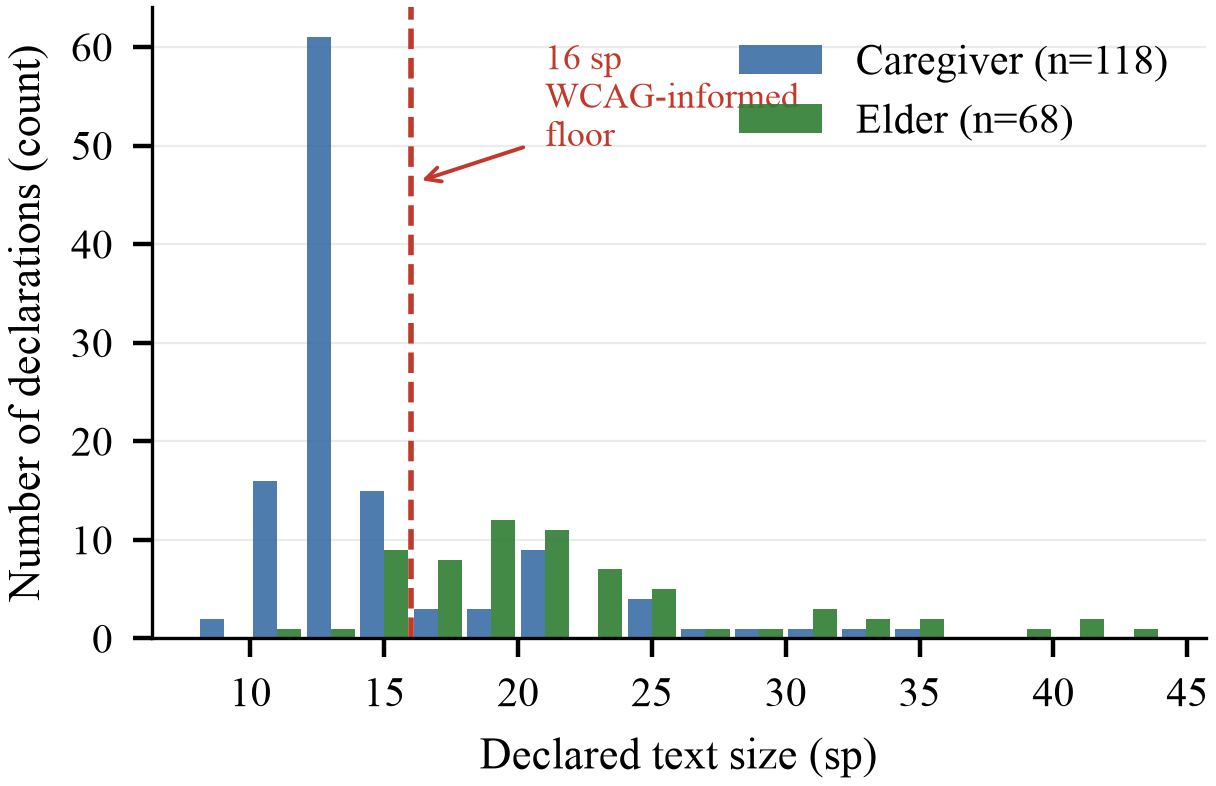
\includegraphics[width=0.58\textwidth]{fig_typescale.png}
\caption{Distribution of declared text sizes across the two surfaces, parsed from source.
Medians are 13\,sp (caregiver) and 20\,sp (elder).}
\label{fig:type}
\end{figure}

Fig.~\ref{fig:type} shows every declared text size on each surface. The elder surface has
a median of 20\,sp against 13\,sp for the caregiver surface, and 16.4\% of its
declarations fall below 16\,sp against 79.7\% on the caregiver surface. The residual small
sizes on the elder surface are supporting captions rather than primary content. Because
the elder surface additionally composes a user-selected scale of 1.0, 1.15, or 1.3 with
the operating system's own font scaling, the effective floor rises further when either is
increased.

\begin{figure}[tb]
\centering
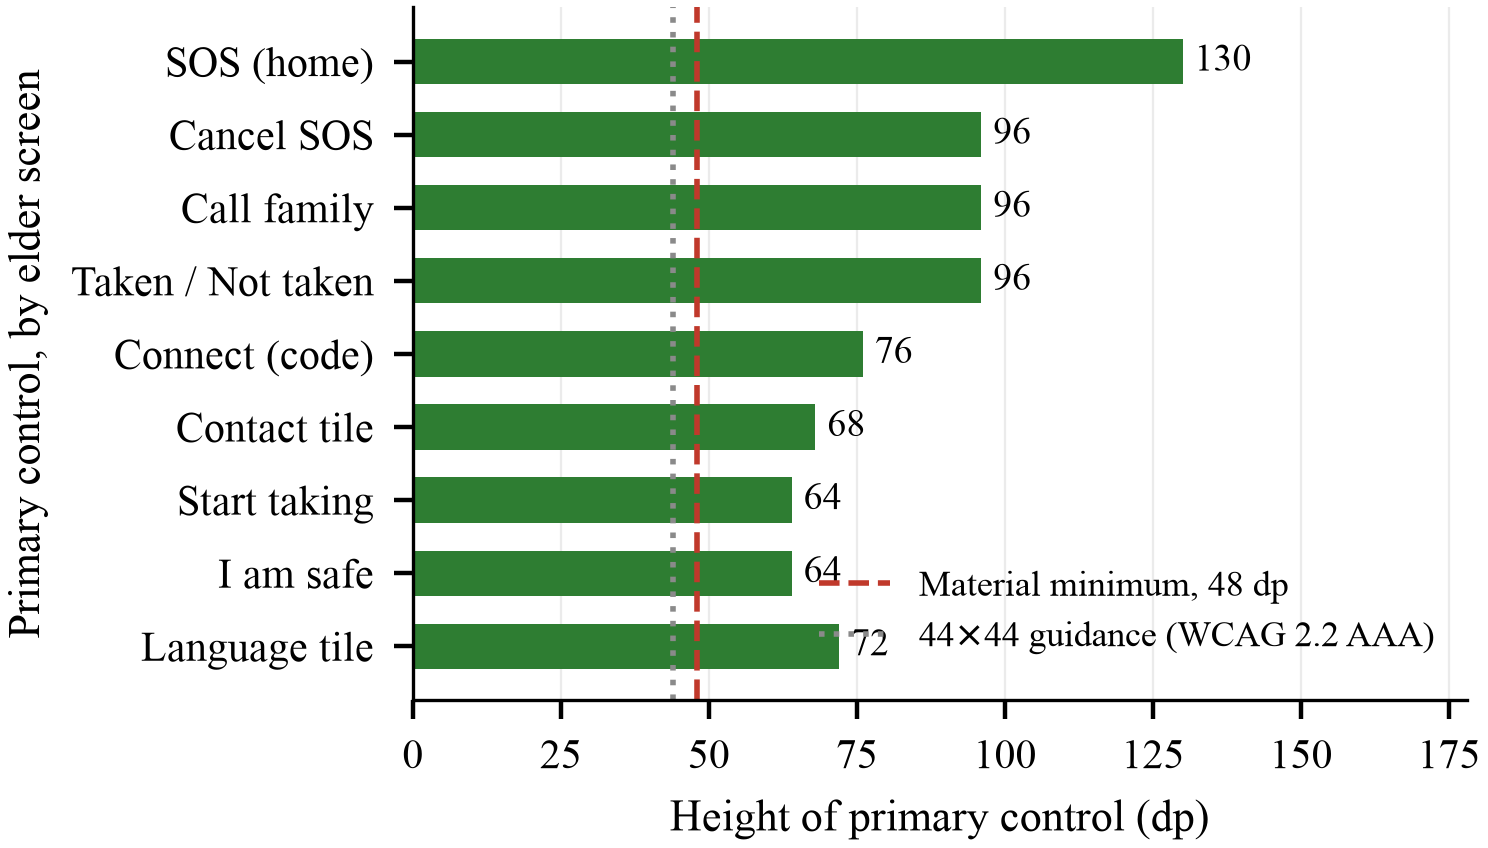
\includegraphics[width=0.58\textwidth]{fig_targets.png}
\caption{Height of the primary control on each elder screen, parsed from source. The
median is 76\,dp and the emergency control is 130\,dp.}
\label{fig:targets}
\end{figure}

Fig.~\ref{fig:targets} reports the height of the primary control on each elder screen. The
smallest is 64\,dp, one third above the 48\,dp platform minimum~\cite{m3}, and comfortably
above the widely cited $44\times44$ target-size recommendation associated with WCAG~2.2
AAA~\cite{wcag}, noting that WCAG is specified in CSS pixels rather than Android
density-independent pixels, so the comparison is indicative rather than exact. The median
is 76\,dp; the emergency control is 130\,dp, roughly 2.7 times the platform minimum.

We state a limit of this measure that a reviewer correctly identified: these are
\emph{declared heights} of the primary control, a one-dimensional static property. They do
not establish the effective touch width, the spacing between adjacent targets, or any
observed user outcome. Meeting a sizing guideline is necessary, not sufficient, and only a
study with older adults can establish sufficiency.

\subsection{Task Interaction Cost}

\begin{figure}[tb]
\centering
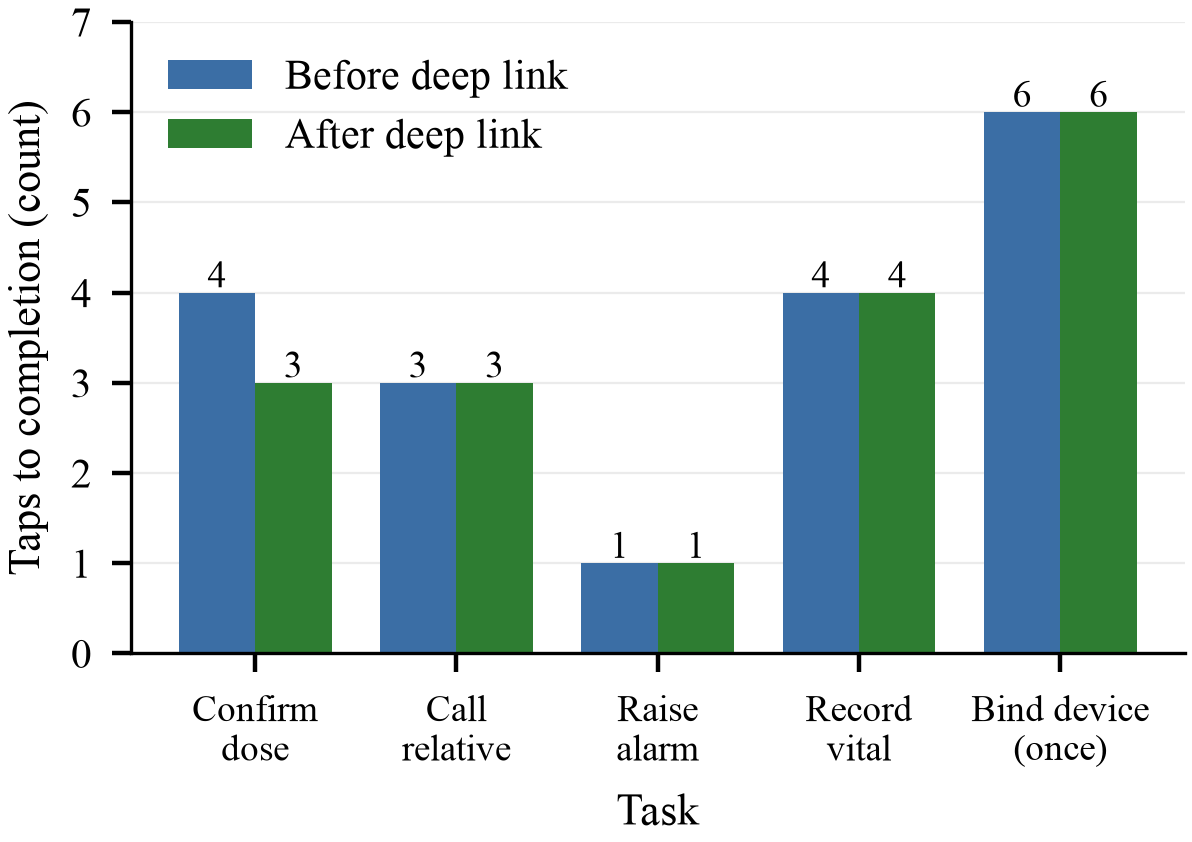
\includegraphics[width=0.58\textwidth]{fig_taps.png}
\caption{Taps to completion for core tasks on the elder surface, counted analytically from
the notification or from the home screen.}
\label{fig:taps}
\end{figure}

Fig.~\ref{fig:taps} counts taps to completion for the elder surface's core tasks. Raising
an alarm costs one tap. Confirming a dose from its reminder costs three, following a
change that routes the notification directly to the medication screen rather than to the
home screen; previously it cost four. The saving is one tap, which sounds trivial and is
not: each intermediate screen is an opportunity for an older adult to lose the thread, and
an unconfirmed dose is recorded as missed and shown to the caregiver as a possible
non-adherence event. Interaction cost on this surface is therefore coupled to data
quality, not only to convenience. These counts are analytic, enumerated by the authors on
the implemented flows; they are not observed task times.

\subsection{Defect Profile: A Single-System Case Study}
\label{sec:defects}

We present this section as a case study of one system audited by its own developers. It is
not a population estimate, and the proportions below should not be read as generalising to
other applications.

After the system was feature-complete and had been exercised on physical devices, we
conducted a structured audit: a line-by-line review of all 83 source files together with
targeted inspection of the database schema and access policies. We recorded every defect
found and classified each by whether a user could have detected it from the interface
alone. Every defect reported here was subsequently corrected, and each correction is
traceable to a commit in the project's version-control history together with the
regression test added for it.

\begin{figure}[tb]
\centering
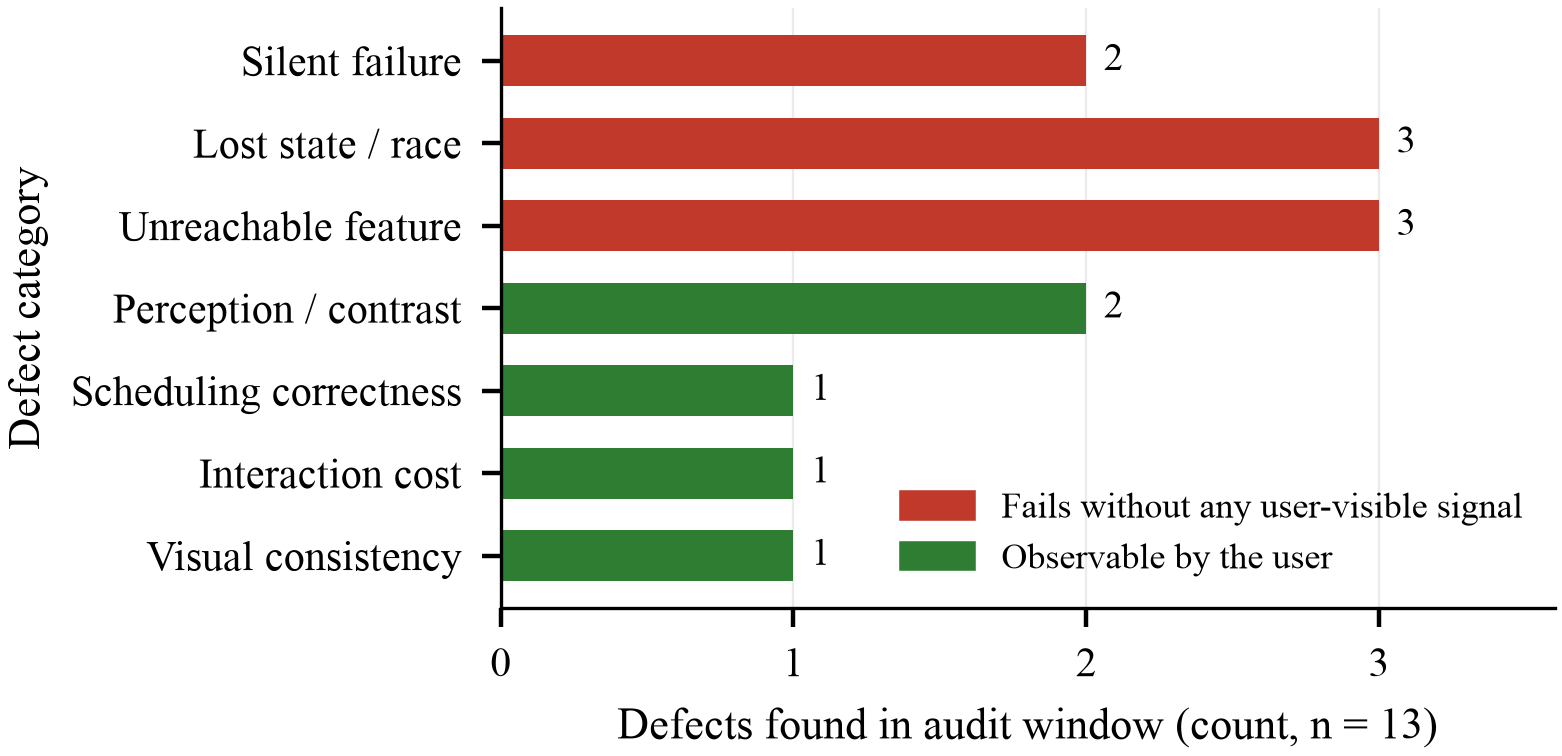
\includegraphics[width=0.58\textwidth]{fig_defects.png}
\caption{Defects found in the audit window, by class. Eight of thirteen would have failed
with no user-visible signal: the interface either reported success or reported nothing.}
\label{fig:defects}
\end{figure}

Thirteen distinct defects were found. Fig.~\ref{fig:defects} gives the distribution. The
dominant finding is that 8 of 13 were silent: the operation failed, or never occurred,
while the interface reported success or reported nothing. Three classes deserve comment.

\begin{itemize}
\item \textbf{Unreachable features (3).} Two complete features --- general reminders for
hydration and activity, and the caregiver invitation path --- were written, exercised by
the caregiver, stored correctly in the database, and delivered to nobody. General
reminders were never armed as alarms on the older adult's device and no server job scanned
for them. The invitation path depended on the telephone-number assumption broken by
federated sign-in (Section~\ref{sec:binding}). In both cases the caregiver's interface
behaved as though the feature worked. Both were subsequently repaired.

\item \textbf{Lost state (3).} Three view models rebuilt their state object when a
background refresh completed, discarding a transient completion flag that the screen used
to navigate. A save that had already succeeded on the server therefore appeared to do
nothing. The defect is timing-dependent, which is why it survived manual testing: it
reproduces only when the refresh completes after the save, most likely on a slow
connection.

\item \textbf{Null failure messages (1 class, 17 sites).} Every repository write terminates
in taking the first element of the server's response. When access policy hides the
returned row, that list is empty and the resulting exception carries no message. Seventeen
call sites propagated that null message directly to the interface, rendering an empty
error and presenting as an unresponsive button.
\end{itemize}

Two observations are candidates for transfer beyond this system, offered as hypotheses
rather than findings. First, identity-model migration produces latent dead features.
Moving from telephone-number authentication to federated sign-in silently invalidated
every code path that used a telephone number as a join key. Nothing failed loudly; two
features simply stopped being reachable. Any system migrating to federated identity should
audit its non-authentication uses of the prior identifier. Second, unit test suites do not
detect unreachable features. Our 142 tests passed throughout the period in which two
features delivered nothing, because each tested component behaved correctly in isolation.
The defect lay in the absence of a caller. Detection required tracing each data type from
producer to consumer.

\subsection{Deployability}
The application declares eleven permissions, none of them in a restricted group. Two
restricted permissions present in an earlier revision were removed in favour of the
user-mediated path of Section~\ref{sec:perm}. The release artefact is 20\,MB and targets
the currently required API level. The permission model was designed to remain compatible
with current Google Play policy; the application has not been published to the store.

\subsection{Threats to Validity}
\label{sec:threats}

The defect study has a single observer and no inter-rater agreement, so the classification
carries the authors' judgement and the authors are the system's developers. Both the
classification boundary (``silent'' versus ``visible'') and the decision of what counts as
one defect were applied by that same observer. An independent re-rating of the thirteen
defects, with a reported agreement statistic, is the correct remedy and is in progress; we
report the single-rater result here rather than implying a validation we have not
performed.

The audit window covers the period after feature completion, not the whole development
history, so the reported count is not a defect density for the project. Conformance
measurements are static properties of the source and say nothing about perception or
comprehension. Tap counts are analytic. Finally, the evaluation contains no systematic
fault injection: we have not exercised lost connectivity, denied runtime permissions, Doze
enforcement, device reboot, or concurrent code redemption under controlled conditions. The
protocol for that suite is defined and is the immediate next step; its absence is why the
dependability claims in this paper are claims about \emph{design discipline} and not about
measured robustness.

\section{Discussion}

\subsection{Silence Is the Dominant Risk}
The audit's central result is that most defects in this feature-complete care application
were invisible from the interface. This has a specific consequence for elder care that it
does not have for, say, a photo application. The older adult often cannot diagnose a
silent failure, and the caregiver --- the person who could --- is looking at a different
device that is also reporting success. A missing reminder produces no artefact at all; its
absence is indistinguishable from a day with no medication due. The system's own adherence
record, which the caregiver trusts, will attribute the gap to the older adult.

We therefore propose that care systems adopt an explicit honesty discipline: acknowledge
only observed outcomes, and name in the interface which outcome was observed; give every
failure path a message a lay reader can act on; and, for any feature whose value is
delivery, test the delivery rather than the storage.

\subsection{Asymmetry as an Accessibility Budget}
The measured gap between the two surfaces is not the result of applying guidelines harder
on one screen. It is a consequence of removing work from that screen. Type size and target
size compete with information density; a surface that must present a scheduling form
cannot also give every control 96\,dp. By moving all configuration to the caregiver, the
elder surface gains an accessibility budget it can spend on sizing and shallow navigation.
We suggest this reframing --- asymmetry as a budget rather than as simplification --- is
the transferable idea, and we are explicit that it is a design insight rather than a new
algorithm.

\subsection{Policy as a Design Input}
Application-store permission policy determined the architecture of our emergency path.
This is unusual to state in a research paper and, we think, ought not to be. A design that
cannot be distributed cannot accumulate the longitudinal evidence the field needs.

\section{Scalability Considerations and Path to Evaluation}

The architecture is designed to support independent care circles: circles are disjoint,
queries are scoped to a profile, and no routine operation requires a cross-tenant scan, so
growth in the number of circles should be horizontal. The heaviest recurring server task is
a scheduled scan for unanswered doses, whose cost is proportional to active profiles with
due doses rather than to total users. Large-scale performance has not been benchmarked;
this is architectural analysis rather than measurement.

Three properties keep per-user cost low. Reminder scheduling is performed on the device, so
the server is not a timing authority and carries no per-dose timer. Adherence writes are
small, append-only, and queue locally when offline. Media is limited to a few profile and
medication photographs per circle. The identified scaling risks are ordinary rather than
architectural: push-token churn requires re-synchronisation on session restore, which we
implement; a single scheduled scan is a single point of failure and would need
partitioning; and per-row policy evaluation grows with policy count, currently thirty-three
across seventeen tables.

\subsubsection{Path to evaluation.} The immediate next step is not a feature. It is
measurement, in two stages. First, a fault-injection suite on physical devices covering
lost connectivity, denied permissions, Doze enforcement, reboot, and concurrent and
repeated code redemption, with the honesty invariant checked automatically in each case.
Second, a small formative study with older adult--caregiver dyads --- as a reviewer of this
work suggested --- measuring delivery-level outcomes the literature usually assumes:
proportion of scheduled reminders actually presented by the device, time from alarm
activation to caregiver acknowledgement, and frequency of the degraded emergency path.
These are precisely the quantities our instrumentation can record truthfully, which is the
point of building it that way.

\section{Limitations}
\label{sec:limits}

We state these plainly because the paper's credibility depends on it.

\begin{itemize}
\item \textbf{No user study has been conducted.} No older adult or caregiver outside the
development team has used the system under observation. We make no usability, adherence, or
clinical claim. Every conformance number in Section~\ref{sec:conf} is a static property of
the implementation.

\item \textbf{No field measurement of delivery.} Reminder delivery has been verified on
physical devices anecdotally and in a shadowed runtime exhaustively, but we have no
distribution of delivery latency across manufacturers and power-management regimes.

\item \textbf{No independent rating, and no fault injection.} The defect taxonomy comes
from one application audited by its own developers, with a single rater
(Section~\ref{sec:threats}). The binding primitive has not been adversarially tested
(Section~\ref{sec:binding}).

\item \textbf{Scope is ageing, not disability in general.} The design and the evaluation
address older adults. We have not evaluated the system with users who have motor, visual,
cognitive, or hearing impairments arising independently of ageing, and we make no claim of
general accessibility.

\item \textbf{Localisation is untested with native speakers.} The four language tables are
complete and machine-checked for structural integrity, but have not been reviewed by native
speakers for register or clarity for older readers.

\item \textbf{Not a medical device.} The system provides no diagnostic or dosing advice.
Vital-sign banding is presented as general reference information only.
\end{itemize}

\section{Conclusion}

We presented CareCompanion, a caregiver-mediated elder-care system built on three
commitments: an asymmetric dual-surface architecture that buys the older adult an
accessibility budget by removing configuration from their device; out-of-band device
binding that repairs an identity gap federated sign-in introduces; and fail-honest
alerting, under which the interface never asserts an outcome it has not observed.

Our measurements show the asymmetry is real --- a median 20\,sp against 13\,sp, every
primary control at or above 64\,dp --- and our case study shows why the honesty discipline
matters: 8 of 13 defects in a feature-complete system would have failed without any
user-visible signal, including two features stored faithfully and delivered to nobody.
That the discipline's own reference implementation still overstated what it had observed,
until review caught it, is the sharpest evidence we can offer that stating the observed
event explicitly must be a design requirement rather than an aspiration. These results
suggest that elder-care systems should be evaluated not only for accessibility and
functionality, but also for whether users receive truthful feedback when critical
operations fail.

\subsubsection{Artifact availability.}
The manuscript, the measurement scripts that generate every figure in
Section~\ref{sec:conf}, and the raw observation files are archived on Zenodo under the
concept DOI \texttt{10.5281/zenodo.23601398}, which always resolves to the latest version.

\subsubsection{\ackname} We thank the anonymous reviewers, whose comments materially
changed Sections~\ref{sec:binding}, \ref{sec:honest} and~\ref{sec:threats}.

\begin{thebibliography}{21}

\bibitem{unfpa}
United Nations Population Fund: India Ageing Report 2023: Caring for Our Elders ---
Institutional Responses. UNFPA India, New Delhi (2023)

\bibitem{dfi}
Data for India: Access to phones and the internet (2025).
\url{https://www.dataforindia.com/comm-tech/}

\bibitem{chakraborty}
Chakraborty, D., Garg, C.: Navigating technology: mobile media usage and reticence among
older adults in rural India. Mobile Media \& Communication \textbf{14}, 31--49 (2025)

\bibitem{khare}
Khare, A., Mukherjee, R., Bedarkar, M.: Beyond digital literacy: a structural model
analysis of technology acceptance among elderly persons. Humanities and Social Sciences
Communications \textbf{13}, 794 (2026)

\bibitem{poor}
Poorcheraghi, H., Negarandeh, R., Pashaeypoor, S., Jorian, J.: Effect of using a mobile
drug management application on medication adherence and hospital readmission among elderly
patients with polypharmacy: a randomized controlled trial. BMC Health Services Research
\textbf{23}, 1192 (2023)

\bibitem{salmensuu}
Salmensuu, O., Isotalo, J., Rijken, M., Hyttinen-Huotari, V., Kaarakainen, M., Linnosmaa,
I.: Effects of using medication reminder technologies by home-dwelling older citizens: a
systematic review. Age and Ageing \textbf{55}(2), afag007 (2026)

\bibitem{awan}
Awan, M., Ali, S., Ali, M., Abrar, M.F., Ullah, H., Khan, D.: Usability barriers for
elderly users in smartphone app usage: an analytical hierarchical process-based
prioritization. Scientific Programming \textbf{2021}, 2780257 (2021)

\bibitem{elguera}
Elguera Paez, L., Zapata Del R\'io, C.: Elderly users and their main challenges usability
with mobile applications: a systematic review. In: Design, User Experience, and Usability.
LNCS, pp. 423--438. Springer, Cham (2019)

\bibitem{liu}
Liu, N., Yin, J., Tan, S.S.-L., Ngiam, K.Y., Teo, H.H.: Mobile health applications for
older adults: a systematic review of interface and persuasive feature design. Journal of
the American Medical Informatics Association \textbf{28}, 2483--2501 (2021)

\bibitem{gomez}
Gomez-Hernandez, M., Ferre, X., Moral, C., Villalba-Mora, E.: Design guidelines of mobile
apps for older adults: systematic review and thematic analysis. JMIR mHealth and uHealth
\textbf{11}, e43186 (2023)

\bibitem{amouzadeh}
Amouzadeh, E., Dianat, I., Faradmal, J., Babamiri, M.: Optimizing mobile app design for
older adults: systematic review of age-friendly design. Aging Clinical and Experimental
Research \textbf{37}, 248 (2025)

\bibitem{quinn}
Quinn, C.C., Staub, S., Barr, E., Gruber-Baldini, A.: Mobile support for older adults and
their caregivers: dyad usability study. JMIR Aging \textbf{2}(1), e12276 (2019)

\bibitem{benmessaoud}
Benmessaoud, C., Pfisterer, K.J., De Leon, A., Saragadam, A., El-Dassouki, N., Young,
K.G.M., Lohani, R., Xiong, T.: Design of a dyadic digital health module for chronic disease
shared care: development study. JMIR Human Factors \textbf{10}, e45035 (2023)

\bibitem{doze}
Android Developers: Optimize for Doze and App Standby.
\url{https://developer.android.com/training/monitoring-device-state/doze-standby}

\bibitem{wiecek}
Wiecek, E., Taylor, S., Rourke, H., Hammond, F., Amador-Fernandez, N.: Mobile health apps
for older adults: real-world evidence on engagement and medication adherence. Frontiers in
Digital Health \textbf{8}, 1716880 (2026)

\bibitem{nimman}
Nimmanterdwong, Z., Boonviriya, S., Tangkijvanich, P.: Human-centered design of mobile
health apps for older adults: systematic review and narrative synthesis. JMIR mHealth and
uHealth \textbf{10}(1), e29512 (2022)

\bibitem{hamill}
Hamill, M., Young, V., Boger, J., Mihailidis, A.: Development of an automated speech
recognition interface for personal emergency response systems. Journal of NeuroEngineering
and Rehabilitation \textbf{6}, 26 (2009)

\bibitem{playsms}
Google Play Console Help: Use of SMS or Call Log permission groups.
\url{https://support.google.com/googleplay/android-developer/answer/10208820}

\bibitem{playblog}
Android Developers Blog: Reminder: SMS/Call Log policy changes (2019).
\url{https://android-developers.googleblog.com/2019/01/reminder-smscall-log-policy-changes.html}

\bibitem{m3}
Material Design 3: Accessibility and touch target size.
\url{https://m3.material.io/foundations/accessible-design/patterns}

\bibitem{wcag}
W3C: Web Content Accessibility Guidelines (WCAG) 2.2. W3C Recommendation (2023).
\url{https://www.w3.org/TR/WCAG22/}

\end{thebibliography}
\end{document}
